% Standalone vector figure extracted from manuscript.tex.
% Rebuild all figures from the project root: bash tkz/build.sh
\documentclass[tikz,border=2pt,class=IEEEtran]{standalone}
\usepackage{amsmath,amssymb,amsfonts}
\usepackage{xcolor}
\usetikzlibrary{positioning,arrows.meta,calc,backgrounds}

% Match the manuscript's IEEE Access text and math font settings.
\renewcommand{\textbf}[1]{{\fontseries{b}\selectfont #1}}
\renewcommand{\textit}[1]{{\itshape #1}}
\makeatletter
\AtBeginDocument{%
  \fontencoding{T1}\rmfamily\fontseries{m}\fontsize{10}{12}\selectfont
  \gdef\operator@encoding{T1}%
  \gdef\encodingdefault{T1}}
\makeatother

% ---- shared palette for review figures ----
\definecolor{cVLA}{HTML}{34618E}   % VLA lane / policy blue
\definecolor{cWM}{HTML}{9E4A3F}    % world-model lane
\definecolor{cCONV}{HTML}{5E4B8B}  % convergence purple
\definecolor{cGood}{HTML}{3A7D44}  % verified green
\definecolor{cWarn}{HTML}{B07A2A}  % caution amber
\definecolor{cPale}{HTML}{F2F0EA}  % pale panel fill
\tikzset{
  fnode/.style={draw=black!55, fill=white, rounded corners=1.5pt,
                inner sep=2.5pt, align=center, font=\fontsize{8}{9.5}\selectfont},
  flane/.style={draw=none, rounded corners=2pt, inner sep=3pt,
                align=center, font=\fontsize{8}{9.5}\selectfont\bfseries, text=white},
  farr/.style={-{Stealth[length=2mm]}, thick, black!60},
}


\newcommand{\figfont}{\fontsize{8}{9.5}\selectfont}

\begin{document}

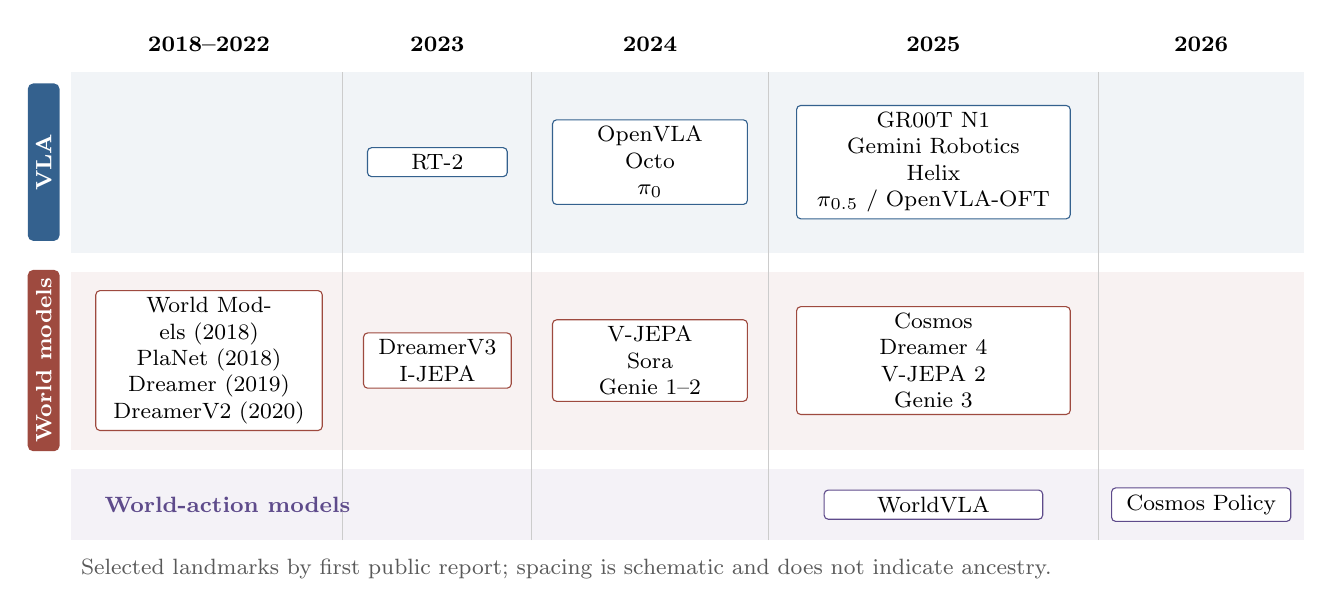
\begin{tikzpicture}[font=\figfont]
% Dates refer to the first public paper/report, not later venue publication.
% Independent landmarks: no arrows assert architectural ancestry.
\foreach \lab/\x in {{2018--2022}/2.1,2023/5.0,2024/7.7,2025/11.3,2026/14.7}{
 \node[font=\figfont\bfseries] at (\x,5.5) {\lab};}
\begin{scope}[on background layer]
\fill[cVLA!7] (0.35,2.85) rectangle (16,5.15);
\fill[cWM!7] (0.35,0.35) rectangle (16,2.6);
\fill[cCONV!7] (0.35,-0.8) rectangle (16,0.1);
\end{scope}
\foreach \x in {3.8,6.2,9.2,13.4}{\draw[black!20] (\x,-0.8)--(\x,5.15);}
\node[flane,fill=cVLA,rotate=90,minimum width=20mm] at (0,4.0) {VLA};
\node[flane,fill=cWM,rotate=90,minimum width=20mm] at (0,1.48) {World models};
\node[font=\figfont\bfseries,cCONV,align=left,anchor=west] at (0.65,-0.35) {World-action models};
\node[fnode,draw=cVLA,text width=16mm] at (5,4) {RT-2};
\node[fnode,draw=cVLA,text width=23mm] at (7.7,4) {OpenVLA\\Octo\\$\pi_0$};
\node[fnode,draw=cVLA,text width=33mm] at (11.3,4) {GR00T N1\\Gemini Robotics\\Helix\\$\pi_{0.5}$ / OpenVLA-OFT};
\node[fnode,draw=cWM,text width=27mm] at (2.1,1.48) {World Models (2018)\\PlaNet (2018)\\Dreamer (2019)\\DreamerV2 (2020)};
\node[fnode,draw=cWM,text width=17mm] at (5,1.48) {DreamerV3\\I-JEPA};
\node[fnode,draw=cWM,text width=23mm] at (7.7,1.48) {V-JEPA\\Sora\\Genie 1--2};
\node[fnode,draw=cWM,text width=33mm] at (11.3,1.48) {Cosmos\\Dreamer 4\\V-JEPA 2\\Genie 3};
\node[fnode,draw=cCONV,text width=26mm] at (11.3,-0.35) {WorldVLA};
\node[fnode,draw=cCONV,text width=21mm] at (14.7,-0.35) {Cosmos Policy};
\node[black!65,align=left,anchor=west] at (0.35,-1.17) {Selected landmarks by first public report; spacing is schematic and does not indicate ancestry.};
\end{tikzpicture}
\end{document}
